\PassOptionsToPackage{table}{xcolor}
\documentclass[a4paper]{article}

%% Language and font encodings
\usepackage[english]{babel}
\usepackage[utf8x]{inputenc}
\usepackage[T1]{fontenc}

%% Sets page size and margins
\usepackage[a4paper,top=3cm,bottom=2cm,left=3cm,right=3cm,marginparwidth=1.75cm]{geometry}

%% Useful packages
\usepackage{amsmath}
\usepackage{graphicx}
\usepackage[colorinlistoftodos]{todonotes}
\usepackage[colorlinks=true, allcolors=blue]{hyperref}
\usepackage{scrextend} % lists
\usepackage{float}
\addtokomafont{labelinglabel}{\bfseries}
%\usepackage{natbib}

\title{Music recomendation}
\author{Raquel Leandra Pérez Arnal y Adrián Sánchez Albanell}
\date{} % Sin fecha.

\definecolor{light-gray}{gray}{0.95}

\begin{document}
\begin{titlepage}
	\centering
	{\scshape\LARGE Grado en Ingenieria Informatica - UPC \par}
	\vspace{1cm}
	{\scshape\Large Proyecto Aprendizaje Autónomo (APA)\par}
	\vspace{1.5cm}
	{\huge\bfseries KKBox's Music Recommendation Challenge\par}
	\vspace{2cm}
	{\Large\itshape Raquel Leandra Pérez Arnal\par}
	{\Large\itshape Adrián Sánchez Albanell\par}
\end{titlepage}
\clearpage
{\hypersetup{linkcolor=black}
\tableofcontents
}
\cleardoublepage

\section{Descripción del trabajo}


\subsection{Introducción}

Este trabajo consiste en elegir un problema de regresión o clasificación y generar un modelo para resolverlo. Para ello usaremos algunos de los métodos, lineales y no lineales, vistos en clase durante el curso de Aprendizaje Autónomo.\\

Hemos elegido un problema de \href{https://www.kaggle.com/competitions}{kaggle competitions} sobre recomendación de música llamado \href{https://www.kaggle.com/c/kkbox-music-recommendation-challenge}{WSDM - KKBox's Music Recommendation Challenge}. Este consiste en un conjunto de datos, proporcionado por \href{https://www.kkbox.com/intl/index.php?area=intl}{KKBOX} - servició de streaming de música asiático - con información sobre diferentes canciones, usuarios y como ha sido el acceso de los usuarios a dichas canciones.\\

Nuestro objetivo es predecir si un usuario que ha escuchado una canción lo volverá a hacer en un periodo de tiempo determinado, por lo tanto se trata de un problema de clasificación binaria: si el usuario volverá a escuchar o no una canción que ya ha oído anteriormente.


\subsection{Conjunto de datos disponible}

Kaggle nos ha proporcionado los datos en seis ficheros con formato CSV, de los cuales usaremos cuatro para la práctica. Los dos restantes són un conjunto de datos de muestra sobre como enviar los datos para el concurso y los datos de test para el concurso (que no nos sirven ya que no tienen la variable target).

\subsubsection*{train.csv}

Contiene la información de las reproducciones de canciones por parte del usuario. Tiene las siguientes variables:

\begin{labeling}{source\_screen\_name}
\item [msno] identificador del usuario.
\item [song\_id] identificador de la canción.
\item [source\_system\_tab] nombre de la pestaña donde se selecciono el evento.\\
Ejemplos: \textit{my library}, \textit{search}, etc.
\item [source\_screen\_name] nombre de la pantalla que ve el usuario.
\item [source\_type] des de donde se ha reproducido la canción.\\
Ejemplos: \textit{album}, \textit{online-playlist}, \textit{song}, etc.
\item [target] variable de target. Si el usuario ha escuchado la canción más de una vez en un intervalo de un mes target es 1, si no es 0.
\end{labeling}

\subsubsection*{members.csv}

Contiene información de los usuarios. Tiene las siguientes variables:

\begin{labeling}{registration\_init\_time}
\item [msno] identificador del usuario.
\item [city] identificador de ciudad.
\item [bd] edad del usuario. Contiene valores outlier.
\item [gender] genero del usuario. Puede ser \textit{female} o \textit{male}.
\item [registered\_via] identificador del método de registro de usuario.
\item [registration\_init\_time] día del registro de usuario, en formato \textit{\%Y\%m\%d}.
\item [expiration\_date] día de expiración del registro de usuario, en formato \textit{\%Y\%m\%d}.
\end{labeling}

\subsubsection*{songs.csv}

Contiene información de las canciones. Tiene las siguientes variables:

\begin{labeling}{song\_length}
\item [song\_id] identificador de la canción.
\item [song\_length] duración de la canción en milisegundos.
\item [genre\_ids] género musical de la canción. Hay canciones con más de un genero, donde el carácter | hace de separador.
\item [artist\_name] nombre del artista.
\item [composer] nombre del compositor o compositores. Si hay más de uno el carácter | hace de separador.
\item [lyricist] nombre del escritor o escritores de la canción. Si hay más de uno el carácter | hace de separador.
\item [language] identificador del lenguaje de la canción.
\end{labeling}

\subsubsection*{song\_extra\_info.csv}

Contiene información extra de las canciones. Tiene las siguientes variables:

\begin{labeling}{song\_name}
\item [song\_id] identificador de la canción.
\item [song\_name] nombre de la canción.
\item [isrc] \href{https://en.wikipedia.org/wiki/International_Standard_Recording_Code}{International Standard Recording Code}. En teoría se puede usar como identificador de la canción, pero hay codigos ISRC sin verificar. Contiene información de la canción aunque puede ser erronea o confusa como el country code, que no se refiere a la canción si no a la agencia que proporciona el codigo ISRC.
\end{labeling}

\subsection{Notas sobre el lenguaje de programación escogido, Python}

El lenguaje de programación usado para realizar esta práctica tenía que ser R. Sin embargo pronto nos dimos cuenta de que, debido al tamaño de los datos de muestra, nuestro desconocimiento de como usarlo para trabajar con grandes cantidades de datos eficientemente y el material de que disponemos, nos iba a ser imposible trabajar con este lenguaje.\\

Debido a esto, hemos decidido usar Python, lenguaje muy usado en Machine Learning y con muchos recursos para trabajar comodamente en este ambito. Python es bastante más eficiente que R gestionando memória y más rápido en cuanto a tiempo de ejecución.\\

Usar Python no ha solucionado todos los problemas generados por tener tantos datos, pero nos ha permitido trabajar mejor y realizar muchas cosas que con R nos habrian sido o imposibles o muy dificiles.


\section{Trabajo Relacionado}

%\section{Posibles Métodos}
%\begin{itemize}
%\item logistic regression, multinomial regression
%(single-layer MLP), LDA, QDA, RDA, \textbf{Naive Bayes}, \textbf{nearest-neighbours},\textbf{linear SVM}, quadratic SVM
%\item one-hidden-layer MLP, the RBFNN, the SVM with RBF kernel, a
%Random Forest
%\end{itemize}


\section{Análisis y preprocesamiento de los datos}

\subsection{Análisis inicial de los datos}

Partiendo de los datos iniciales (descritos en el apartado \textit{Conjunto de datos disponible}) hemos generado un solo data frame uniendo primero la información de \textbf{members} y \textbf{train} por \textit{msno}, y luego uniendo el resultado a \textbf{songs} y \textbf{song\_extra\_info} por \textit{song\_id}. Al nuevo conjunto de datos con toda la información lo llamaremos \textbf{merged}. El nuevo conjunto de datos se compone de $20$ variables y $7377418$ muestras diferentes. La siguiente tabla nos muestra información sobre los valores perdidos en cada variable y su tipo:
\begin{table}[H]
\centering
\rowcolors{1}{white}{light-gray}
\begin{tabular}{l*{4}l}
\hiderowcolors
\textbf{Variable}          & \textbf{Valores perdidos} & \textbf{Porcentaje}  & \textbf{Tipo de datos} \\
\showrowcolors
\hline 
\textbf{msno}                     & 0                 & 0           & categóricos (object)                    \\
\textbf{song\_id}                 & 0                 & 0           & categóricos (object)                    \\
\textbf{source\_system\_tab}      & 24849             & 0.3368      & categóricos (object)                    \\
\textbf{source\_screen\_name}     & 414804            & 5.6226      & categóricos (object)                    \\
\textbf{source\_type}             & 21539             & 0.2919      & categóricos (object)                    \\
\textbf{target}                   & 0                 & 0           & categóricos (uint8)                     \\
\textbf{city}                     & 0                 & 0           & categóricos (int64)                     \\
\textbf{bd}                       & 0                 & 0           & numéricos (int64)                       \\
\textbf{gender}                   & 2961479           & 40.142      & categóricos (object)                    \\
\textbf{registered\_via}          & 0                 & 0           & categóricos (int64)                     \\
\textbf{registration\_init\_time} & 0                 & 0           & numéricos (int64) (\textit{\%Y\%m\%d})  \\
\textbf{expiration\_date}         & 0                 & 0           & numéricos (int64) (\textit{\%Y\%m\%d})  \\
\textbf{song\_length}             & 114               & 0.0015      & numéricos (float64)                     \\
\textbf{genre\_ids}               & 118455            & 1.605       & categóricos (object)                    \\
\textbf{artist\_name}             & 114               & 0.0015      & categóricos (object)                    \\
\textbf{composer}                 & 1675706           & 22.7139     & categóricos (object)                    \\
\textbf{lyricist}                 & 3178798           & 43.0882     & categóricos (object)                    \\
\textbf{language}                 & 150               & 0.0020      & categóricos (float64)                   \\
\textbf{name}                     & 1457              & 0.0197      & categóricos (object)                    \\
\textbf{isrc}                     & 577858            & 7.8327      & categóricos (object)                    \\
\end{tabular}
\caption{\textit{Información general sobre el conjunto de datos merged.}}
\end{table}
En la tabla siguiente vemos de cuantas categorías consta cada variable categórica. Esto es muy importante en nuestro caso porque contamos con un conjunto de datos muy grande y el número de categorías añade mucha complejidad a los datos cuando queramos diseñar los diferentes modelos:
\begin{table}[H]
\centering
\rowcolors{1}{white}{light-gray}
\begin{tabular}{l*{2}l}
\hiderowcolors
\textbf{Variable}                   & \textbf{Número de categorías} \\
\showrowcolors
\hline 
\textbf{msno}                     & 30755   \\
\textbf{song\_id}                 & 359966  \\
\textbf{source\_system\_tab}      & 8       \\
\textbf{source\_screen\_name}     & 20      \\
\textbf{source\_type}             & 12      \\
\textbf{target}                   & 2       \\
\textbf{city}                     & 21      \\
\textbf{gender}                   & 2       \\
\textbf{registered\_via}          & 5       \\
\textbf{genre\_ids}               & 166     \\
\textbf{artist\_name}             & 40582   \\
\textbf{composer}                 & 81566   \\
\textbf{lyricist}                 & 38473   \\
\textbf{language}                 & 10      \\
\textbf{name}                     & 234144  \\
\textbf{isrc}                     & 269760  \\
\end{tabular}
\caption{\textit{Número de categorías en las variables categóricas del conjunto de datos.}}
\end{table}
Con esta información pasaremos a tratar los datos para preprocesarlos.

\subsection{Tratamiento de valores perdidos}

\begin{figure}[H]
\centering
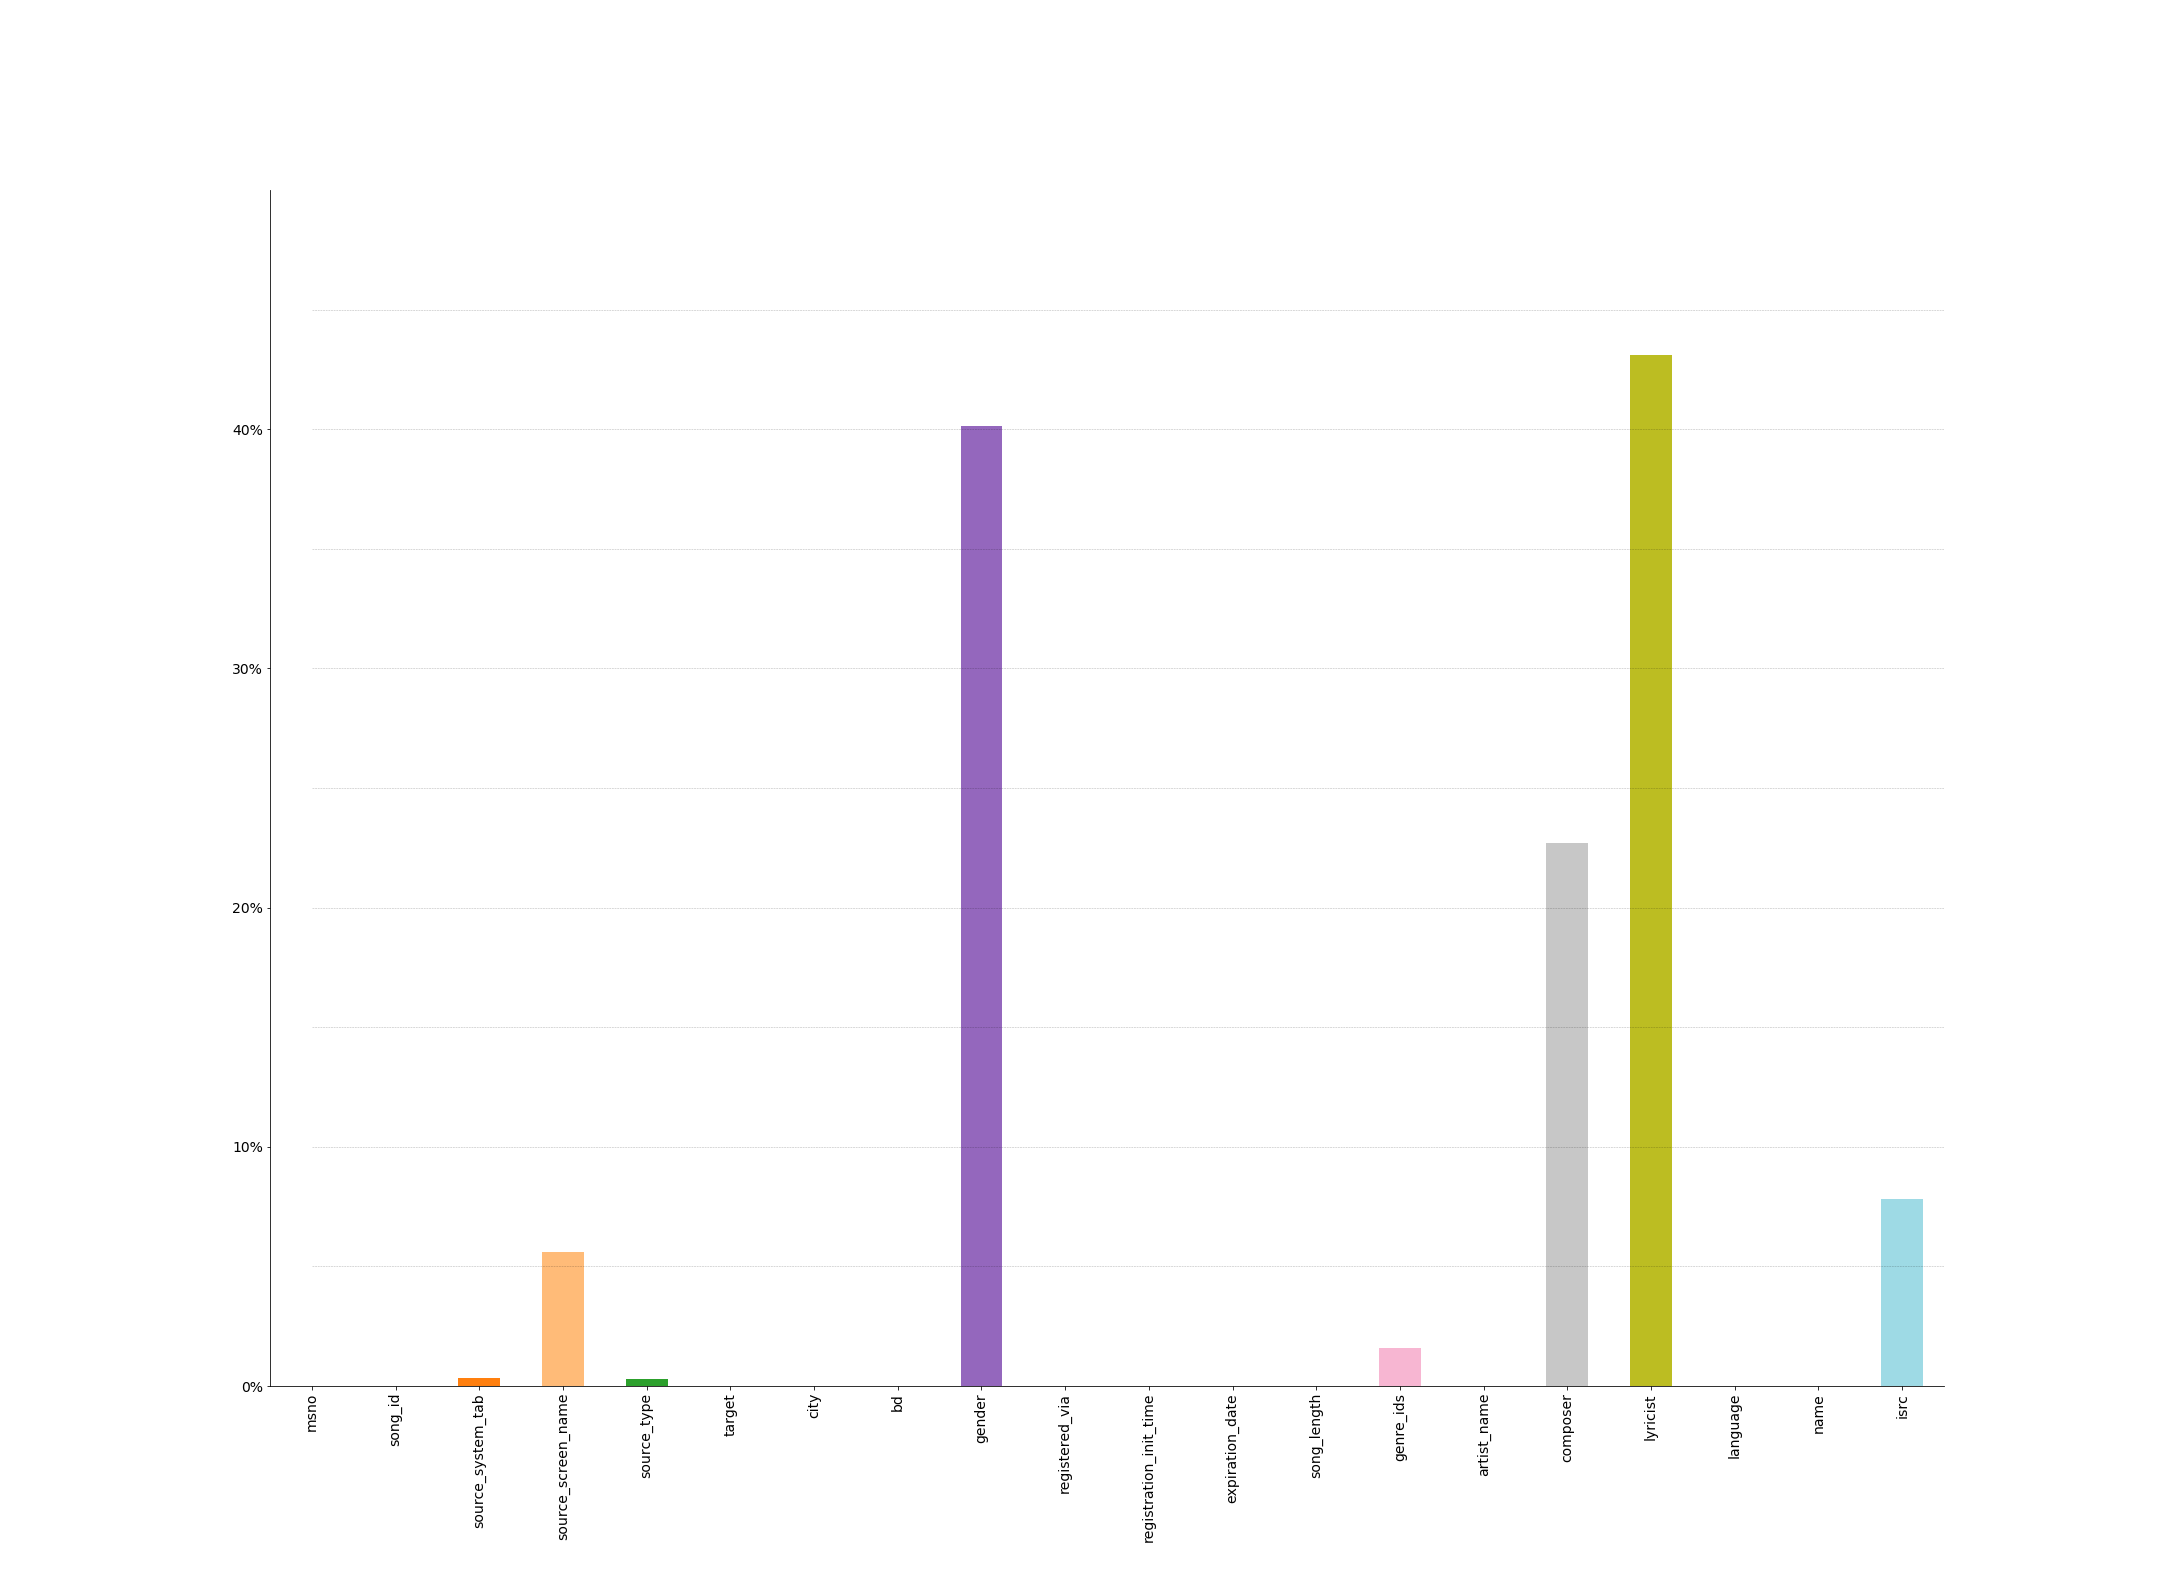
\includegraphics[width=1\textwidth]{Images/lost_values_percent.png}
\caption{\textit{En esta gráfica podemos ver porcentaje de valores perdidos en cada variable del conjunto final de datos.}}
\end{figure}

Como podemos ver en \textit{Table 1} y \textit{Figure 1} tenemos varias variables donde hay valores perdidos y que trataremos de diferentes maneras.\\

\begin{itemize}
\item Las variables \textit{lyricist} y \textit{gender} hemos decidido eliminarlas por tener un porcentaje muy alto de valores perdidos, más de un $40\%$. 
\item La variable \textit{composer} también hemos decidido eliminarla. Aunque el porcentaje de valores perdidos en esta variable es un $22.71\%$, un valor alto pero que podriamos haber decidido imputar por ejemplo, cuenta con $81566$ categorías diferentes. Teniendo en cuenta el tamaño de nuestro conjunto de datos, la complejidad que añade esta variable nos es intratable con el conocimiento y material del que disponemos.
\item El resto de variables tienen menos de un $10\%$ de valores perdidos. Podriamos haberlos imputado a partir del resto de datos, pero disponemos de un conjunto de datos lo bastante grande como para poder eliminar las muestras donde aparecen valores nulos sin problemas.
\end{itemize}
Después de tratar los valores perdidos en el conjunto de datos este consta de 17 variables y $6317407$ muestras.

\subsection{Tratamiento de outliers}

La única variable que contiene outliers es \textit{bd}, que representa la edad de un usuario, y tiene valores imposibles (como 0 años). Lo primero que hemos hecho ha sido eliminarlos, convirtiendo los valores menores a 16 y los mayores a 90 en valores nulos.\\

Habiamos pensado en imputar el valor de los outliers mediante KNN, pero al convertirlos en valores nulos hemos visto que un $39.68\%$ de \textit{bd} són outliers. Al ver esto hemos decidido que lo mejor era simplemente eliminar esta variable.

\subsection{Creación de nuevas variables}

La variable \textit{ISRC} representa el \href{https://en.wikipedia.org/wiki/International_Standard_Recording_Code}{International Standard Recording Code} de la canción. Este codigo tiene un formato de 12 carácteres y cuatro partes de la forma CC-XXX-YY-NNNNN, donde:

\begin{labeling}{source\_screen\_name}
\item [CC] identificador del país del emisor del código ISRC.
\item [XXX] codigo numérico identificador del emisor del código ISRC.
\item [YY] dos últimos digitos del año en que el código ISRC fue asignado a la grabación.
\item [NNNNN] identificador numérico de la grabación.
\end{labeling}

De esta variable crearemos una nueva variable con el año en que se registro el codigo de la grabación, ya que nos ha parecido un valor representativo para el conjunto, a la que llamaremos \textit{song\_year}. Para hacerlo cogeremos los dos dígitos YY del código ISRC, los valores mayores a 18 los convertimos en valores numéricos de la forma 19YY, el resto de la forma 20YY.

\subsection{Selección de features}

Hemos decidido eliminar varias de las variables. En esta sección explicaremos cuales y los motivos principales para hacerlo.
\begin{itemize}
\item \textit{msno} y \textit{song\_id} han sido eliminadas por tratarse de simples identificadores, sin otro objetivo que identificar la muestra o una parte de ella. Se han usado para unir los diferentes conjuntos de datos de que disponiamos inicialmente, pero de cara al análisis no tienen utilidad alguna.
\item El \textit{isrc} es otro identificador como las variables mencionadas anteriormente. Sin embargo contiene más información que podría parecer útil.\\
De esa información ya hemos elegido una parte que se encuentra en la variable \textit{song\_year}, la otra información que podemos encontrar en el ISRC o bien són identificadores (y no nos aportan información relevante) o puede ser erronea (el CC, en la pagina del concurso de kaggle, cuando explican la información de los diferentes ficheros, se avisa de que esta parte del identificador puede resultar confusa o incluso erronea).\\
Por estas razones de esta variable no aprovechamos nada más de lo que pueda aportar y la descartamos.
\item \textit{artist\_name} y \textit{name} las rechazamos porque nos són computacionalmente intratables, tanto en R como en Python. La variable \textit{artist\_name} tiene $40582$ clases diferentes y \textit{name} otras $234144$.
\item \textit{registered\_via}, \textit{registration\_init\_time} y \textit{expiration\_date} nos proporcionan información irrelevante para determinar si un usuario escuchara o no una canción repetidas veces.
\end{itemize}

Después del proceso de selección de features nos quedan $6317407$ muestras y 9 variables, 8 de ellas categóricas y 2 numéricas:

\begin{table}[H]
\centering
\rowcolors{1}{white}{light-gray}
\begin{tabular}{l*{2}l}
\hiderowcolors
\textbf{Variable}                   & \textbf{Número de categorías} \\
\showrowcolors
\hline 
\textbf{source\_system\_tab}      & 8                \\
\textbf{source\_screen\_name}     & 20               \\
\textbf{source\_type}             & 12               \\
\textbf{target}                   & 2                \\
\textbf{city}                     & 21               \\
\textbf{genre\_ids}               & 166              \\
\textbf{language}                 & 10               \\
\textbf{song\_length}             & (no categórica)  \\
\textbf{song\_year}               & (no categórica)  \\
\end{tabular}
\caption{\textit{Número de categorías en las variables categóricas del conjunto de datos.}}
\end{table}

\subsection{Codificación de variables categóricas}

La mayoría de variables categóricas las dejamos como estan, pero \textit{genre\_ids} la preprocesamos para hacer un poco menos complejo el conjunto de datos con el que trataremos luego.
La variable \textit{genre\_ids} permite varias categorías diferentes por muestra (como se explica en la sección \textit{Conjunto de datos disponible}). Hemos tratado los datos para que cada muestra tenga una sola categoría para esta variable.\\

Para hacerlo hemos calculado la freqüencia de cada categoría diferente y hemos tratado cada muestra para que conserve solo la más freqüente de sus categorías.\\

A parte de simplificar las muestras que tenian multiples categorías, después de tratar los datos el número de categorías diferentes en \textit{genre\_ids} se ha reducido de 166 a 148.

\subsection{Estandarización}

\subsection{Transformación de variables}

\section{Protocolo de re-muestreo}

Una vez preprocesados los datos, a la hora de entrenar los métodos hemos separado en dos conjuntos el conjunto de datos 
con el objetivo de poder comparar bien los resultados, obteniendo:

\begin{table}[H]
\centering
\rowcolors{1}{white}{light-gray}
\begin{tabular}{l*{2}l}
\hiderowcolors
\textbf{Subconjunto}              & \textbf{Proporción}   & \textbf{Tamaño}    \\ \hline
\showrowcolors
\hline 
\textbf{Entrenamiento}                     & 0.7                   & 4,422,185   \\
\textbf{Test}                              & 0.3                   & 1,895,222   \\
\textbf{Total}                             & 1                     & 6,317,407   \\
\end{tabular}
\caption{\textit{Particines de entrenamiento y test del conjunto de datos.}}
\end{table}

Con tal cantidad de datos podriamos haber tomado una partición de datos con más entrenamiento y menos test ($90$/$10$ o incluso más por ejemplo), pero hemos elejido particionar los datos en $70\%$ entrenamiento y $30\%$ test por dos razones:
\begin{itemize}
\item Obtener unos resultados más estables a la hora de comparar los distintos modelos.
\item Reducir la cantidad de datos de entrenamiento a una cantidad ligeramente más tratable a nivel computacional. Ya que con tal cantidad de datos la potencia computacional y el tiempo de procesamiento necesarios són bastante considerables. 
\end{itemize}

Además, para algunos modelos hemos tenido que calcular hiper-parámetros. Hemos usado \textit{Random Search Cross-Validation} para ello.\\

Con tal cantidad de datos nos podríamos haber limitado a tomar una partición de validación para buscar los mejores hiper-parámetros, pero de esta forma teníamos que entrenar iterativamente cada modelo con los diferentes hiper-parámetros a comprobar y luego analizar los resultados obtenidos con la partición de validación. El problema en este caso es que cuando había que buscar varios hiper-parámetros para un mismo modelo no sabíamos paralelizar el proceso, y hacerlo de esta forma era significativamente más lento que otras opciones ya implementadas en librerías como la que hemos usado, \textit{sklearn}, como por ejemplo  \textit{sklearn.model\_selection.GridSearchCV} o \textit{sklearn.model\_selection.RandomizedSearchCV}. De estas dos opciones hemos decidido usar \textit{RandomizedSearchCV}.\\

El método \textit{RandomizedSearchCV} de \textit{sklearn} aplica \textit{3-fold stratified cross-validation} a una muestra aleatoria de los hiper-parámetros que queremos obtener. A diferencia del \textit{Grid-Search CV}, este método no prueba todas las posibles opciones, lo que implica una menor cantidad de entrenamientos del modelo y por tanto va más rápido. Esto implica un coste en cuanto a la accuracy respecto al \textit{Grid-Search CV}, sin embargo este coste es negligible. Como se puede ver randomSearch\cite{randomSearch} es especialmente efectivo con conjuntos de validación grandes, como es nuestro caso, y es la mejor opción que hemos encontrado.\\

\section{Resultados de los métodos lineales}

\subsection{Linear Discriminant Analysis}

Hemos elegido este modelo por ser rápido y sencillo. Al no tener hiper-parámetros ha bastado con entrenarlo 
con la partición de train al completo y probarlo con la partición de test. De esta forma nos ha dado los siguientes resultados: 
\begin{table}[H]
\centering
\rowcolors{1}{white}{light-gray}
\begin{tabular}{l*{5}l}
\hiderowcolors
  \textbf{Clase}      & \textbf{Precision}   & \textbf{Recall}   & \textbf{F1-Score}   & \textbf{Support} \\ \hline
\showrowcolors
\hline 
\textbf{0}             & 0.62                & 0.63              &  0.63               &    933345    \\
\textbf{1}             & 0.64                & 0.63              &  0.63               &    961878   \\
\textbf{Average/Total} & 0.63                & 0.63              &  0.63               &   1895223    \\
\end{tabular}
\caption{\textit{Particines de entrenamiento y test del conjunto de datos.}}
\end{table}

Viendo los resultados obtenidos, es probable que los datos no cumplan la hipótesis de homocedasticidad. 

\subsection{Quadratic Discriminant Analysis}

Hemos elegido este modelo por ser rápido y sencillo. Al no tener hiper-parámetros ha bastado con entrenarlo 
con la partición de train al completo y probarlo con la partición de test. De esta forma nos ha dado los siguientes resultados: 
\begin{table}[H]
\centering
\rowcolors{1}{white}{light-gray}
\begin{tabular}{l*{5}l}
\hiderowcolors
  \textbf{Clase}      & \textbf{Precision}   & \textbf{Recall}   & \textbf{F1-Score}   & \textbf{Support} \\ \hline
\showrowcolors
\hline 
\textbf{0}             & 0.62                & 0.54              &  0.57               &    933345    \\
\textbf{1}             & 0.60                & 0.67              &  0.64               &    961878   \\
\textbf{Average/Total} & 0.61                & 0.61              &  0.61               &   1895223    \\
\end{tabular}
\caption{\textit{Particines de entrenamiento y test del conjunto de datos.}}
\end{table}

** Escribir motivos por los que va peor que el LDA

\subsection{Regularized Discriminant Analysis}

Hemos elegido este modelo por ser rápido y sencillo. 

Hemos probado hiperparámetros dentro de una distribución uiniforme en 0,1

Hemos acabado eligiendo: 0.7010416905212281

De esta forma nos ha dado los siguientes resultados: 


\begin{table}[H]
\centering
\rowcolors{1}{white}{light-gray}
\begin{tabular}{l*{5}l}
\hiderowcolors
  \textbf{Clase}      & \textbf{Precision}   & \textbf{Recall}   & \textbf{F1-Score}   & \textbf{Support} \\ \hline
\showrowcolors
\hline 
\textbf{0}             & 0.57                & 0.60              &  0.59               &    933345    \\
\textbf{1}             & 0.59                & 0.56              &  0.58               &    961878   \\
\textbf{Average/Total} & 0.58                & 0.58              &  0.58               &   1895223    \\
\end{tabular}
\caption{\textit{Particines de entrenamiento y test del conjunto de datos.}}
\end{table}

Va mejor que el LDA pero no significativamente.


\section{Resultados de los métodos no lineales}

\subsection{Multi Layer Perceptron}
\begin{table}[H]
\centering
\rowcolors{1}{white}{light-gray}
\begin{tabular}{l*{5}l}
\hiderowcolors
  \textbf{Clase}      & \textbf{Precision}   & \textbf{Recall}   & \textbf{F1-Score}   & \textbf{Support} \\ \hline
\showrowcolors
\hline 
\textbf{0}             & 0.56                & 0.89              &  0.69               &    933345    \\
\textbf{1}             & 0.75                & 0.31              &  0.44               &    961878   \\
\textbf{Average/Total} & 0.66                & 0.60              &  0.56               &   1895223    \\
\end{tabular}
\caption{\textit{Particines de entrenamiento y test del conjunto de datos.}}
\end{table}


Va mejor que el LDA pero no significativamente.

\subsection{Random Forest}
\begin{table}[H]
\centering
\rowcolors{1}{white}{light-gray}
\begin{tabular}{l*{5}l}
\hiderowcolors
  \textbf{Clase}      & \textbf{Precision}   & \textbf{Recall}   & \textbf{F1-Score}   & \textbf{Support} \\ \hline
\showrowcolors
\hline 
\textbf{0}             & 0.67                & 0.66              &  0.66               &    933345    \\
\textbf{1}             & 0.67                & 0.69              &  0.68               &    961878   \\
\textbf{Average/Total} & 0.67                & 0.67              &  0.67               &   1895223    \\
\end{tabular}
\caption{\textit{Particines de entrenamiento y test del conjunto de datos.}}
\end{table}

Va mejor que el LDA pero no significativamente.

\section{Descripción y justificación del modelo escogido}

\section{Conclusiones}

\clearpage
\section{Bibliografía}

\bibliographystyle{unsrt}
\bibliography{biblio}


\end{document}
